%%%%%%%%%%%%%%%%%%%%%%
%%Options for presentations (in-class) and handouts (e.g. print). 
\documentclass[pdf
%,handout
]{beamer}
\usepackage{pgfpages}
%\pgfpagesuselayout{2 on 1}[letterpaper,border shrink=5mm]

\graphicspath{{../}}
%%%%%%%%%%%%%%%%%%%%%%
%% Change this for different slides so it appears in bar
\usepackage{authoraftertitle}
\date{Spectral Theory: 7.1 Eigenvalues and Eigenvectors}

%%%%%%%%%%%%%%%%%%%%%%
%% Upload common style file
\usepackage{../LyryxLinearAlgebraSlidesStyle}

\begin{document}
	
	%%%%%%%%%%%%%%%%%%%%%%%
	%% Title Page and Copyright Common to All Slides	
	%Title Page
	\input ../frontmatter/titlepage.tex	
	%LOTS Page
	%\input frontmatter/lyryxopentexts.tex	
	%Copyright Page
	\input ../frontmatter/copyright.tex	
	%%%%%%%%%%%%%%%%%%%%%%%%%

{\small
\section{Definition}
%-------------- start slide -------------------------------%
\frame{\frametitle{Motivation: Calculating Powers of a Matrix}
\begin{example}
Let $A=
\left[\begin{array}{rr}
4 & -2 \\
-1 & 3
\end{array}\right]$.
Find $A^{100}$.
\pause
\begin{center}
\alert{\large How can we do this efficiently?}
\end{center}
\pause
Consider the matrix
$P=
\left[\begin{array}{rr}
1 & -2 \\
1 & 1
\end{array}\right]$.
\pause
Observe that $P$ is invertible (why?), 
\pause
and that
\[ P^{-1} = 
\frac{1}{3} \left[\begin{array}{rr}
1 & 2 \\
-1 & 1
\end{array}\right].\]
\pause
Furthermore,
\[ P^{-1}AP \pause
= \frac{1}{3} \left[\begin{array}{rr}
1 & 2 \\
-1 & 1
\end{array}\right]
\left[\begin{array}{rr}
4 & -2 \\
-1 & 3
\end{array}\right]
\left[\begin{array}{rr}
1 & -2 \\
1 & 1
\end{array}\right]
\pause
=
\left[\begin{array}{rr}
2 & 0 \\
0 & 5
\end{array}\right] = D,
\]
\pause
where $D$ is a \alert{diagonal} matrix.
\end{example}
}
%-------------- end slide -------------------------------%

%-------------- start slide -------------------------------%
\frame{
\begin{example}[continued]
\pause
This is significant, because
\begin{eqnarray*}
P^{-1} A P & = & D \\
\pause
P(P^{-1} A P)P^{-1} & = & PDP^{-1} \\
\pause
(PP^{-1}) A (PP^{-1}) & = & PDP^{-1} \\
\pause
IAI & = & PDP^{-1} \\
\pause
A & = & PDP^{-1},
\end{eqnarray*}
\pause
and so
\begin{eqnarray*}
A^{100} & = & (PDP^{-1})^{100} \\
\pause
& = & (PDP^{-1})(PDP^{-1})(PDP^{-1}) \cdots (PDP^{-1}) \\
\pause
& = & PD(P^{-1}P)D(P^{-1}P)D(P^{-1} \cdots P)DP^{-1} \\
\pause
& = & PDIDIDI \cdots I DP^{-1} \\
\pause
& = & PD^{100}P^{-1}.
\end{eqnarray*}
\end{example}
}
%-------------- end slide -------------------------------%

%-------------- start slide -------------------------------%
\frame{
\begin{example}[continued]
\pause
Now,
\[ D^{100} =
\left[\begin{array}{rr}
2 & 0 \\
0 & 5
\end{array}\right]^{100}
=
\left[\begin{array}{cc}
2^{100} & 0 \\
0 & 5^{100}
\end{array}\right].\]
\pause
Therefore,
\begin{eqnarray*}
A^{100} \pause & = & PD^{100}P^{-1} \\
\pause
& = & \left[\begin{array}{rr}
1 & -2 \\
1 & 1
\end{array}\right]
\left[\begin{array}{cc}
2^{100} & 0 \\
0 & 5^{100}
\end{array}\right]
\left(\frac{1}{3}\right)
\left[\begin{array}{rr}
1 & 2 \\
-1 & 1
\end{array}\right] \\ \\
\pause
& = &
\frac{1}{3}
\left[\begin{array}{cc}
2^{100} + 2\cdot 5^{100} & 2^{100} - 2\cdot 5^{100} \\
2^{100} - 5^{100} & 2\cdot 2^{100} + 5^{100}
\end{array}\right] \\ \\
\pause
& = &
\frac{1}{3}
\left[\begin{array}{cc}
2^{100} + 2\cdot 5^{100} & 2^{100} - 2\cdot 5^{100} \\
2^{100} - 5^{100} & 2^{101} + 5^{100}
\end{array}\right]
\end{eqnarray*}
\end{example}
}
%-------------- end slide -------------------------------%

%-------------- start slide -------------------------------%
\frame{
\begin{theorem}\em
If $A$ is an $n\times n$ matrix and
$P$ is an invertible $n\times n$ matrix such that
$A=PDP^{-1}$, then $A^k=PD^kP^{-1}$ for each
$k=1,2,3,\ldots$
\end{theorem}
\pause
\bigskip

The process of finding an \alert{invertible} matrix $P$ and
a \alert{diagonal} matrix $D$ so that $A=PDP^{-1}$
is referred to as \alert{diagonalizing} the matrix $A$,
and $P$ is called the \alert{diagonalizing} matrix for $A$.
\bigskip

\pause
\begin{block}{Questions}
\begin{itemize}
\item When is it possible to diagonalize a matrix?
\pause
\item How do we find a diagonalizing matrix?
\end{itemize}
\end{block}
\pause
\begin{alertblock}{Answer}
Eigenvalues and eigenvectors.
\end{alertblock}
}
%-------------- end slide -------------------------------%


%-------------- start slide -------------------------------%
\frame{\frametitle{Eigenvalues and Eigenvectors}
\begin{definition}
Let $A$ be an $n\times n$ matrix, $\lambda$ a real number,
and $\alert{X\neq 0}$ an $n$-vector.
If $AX=\lambda X$, then $\lambda$ is an
\alert{eigenvalue} of $A$, and $X$ is
an \alert{eigenvector} of $A$ corresponding to $\lambda$,
or a \alert{$\lambda$-eigenvector}.
\end{definition}
\pause
\begin{example}
Let $A=
\left[\begin{array}{rr}
1 & 2 \\
1 & 2
\end{array}\right]$ and
$X=\left[\begin{array}{r}
1 \\ 1 \end{array}\right]$.
\pause
Then
\[ AX=\left[\begin{array}{rr}
1 & 2 \\
1 & 2
\end{array}\right]
\left[\begin{array}{r}
1 \\ 1 \end{array}\right]
\pause
=
\left[\begin{array}{r}
3 \\ 3 \end{array}\right]
\pause
=3
\left[\begin{array}{r}
1 \\ 1 \end{array}\right]
\pause
=3X.
\]
\pause
This means that $3$ is an \alert{eigenvalue} of $A$, 
\pause
and
$\left[\begin{array}{r}
1 \\ 1 \end{array}\right]$ is an \alert{eigenvector of
$A$ corresponding to $3$} (or a $3$-eigenvector of $A$).
\end{example}
}
%-------------- end slide -------------------------------%

%-------------- start slide -------------------------------%
\frame{
\begin{block}{What an eigenvalue and eigenvector tell us about a matrix}
Suppose that $A$ is an $n\times n$ matrix, with eigenvalue
$\lambda$ and corresponding eigenvector $X$.
\pause
Then $X\neq 0$ is an $n$-vector, 
$\lambda\in\RR$, and $AX=\lambda X$.
\pause

It follows that
\begin{eqnarray*}
\lambda X - AX & = & 0 \\
\pause
\lambda I X - AX & = & 0 \\
\pause
(\lambda I - A)X & = & 0 
\end{eqnarray*}
\pause
Since $X\neq 0$, $X$ is a nontrivial solution to the
linear system with coefficient matrix $\lambda I-A$, 
\pause
and therefore the matrix \alert{$\lambda I-A$ is not
invertible}.
\pause 
Since a matrix is invertible if and only if its 
determinant is not equal to zero, it follows that
\[ \det(\lambda I - A)=0.\]
%\begin{eqnarray*}
%X &=& IX \\
%&=& ((\lambda I - A)^{-1} (\lambda I - A))X \\
%&=& (\lambda I - A)^{-1} ((\lambda I - A)X)\\
%&=& (\lambda I - A)^{-1} 0 \\
%&=& 0 \\
%\end{eqnarray*}
\end{block}
}
%-------------- end slide -------------------------------%


%-------------- start slide -------------------------------%
\frame{\frametitle{The Characteristic Polynomial}
\begin{definition}
The \alert{characteristic polynomial} of an $n\times n$ matrix $A$ is
defined to be
\[ \alert{c_A(x)=\det(xI-A).}\]
\end{definition}
\pause
\begin{example}
The characteristic polynomial of
$A=\left[\begin{array}{rr}
4 & -2 \\ -1 & 3
\end{array}\right]$ 
\pause 
is
\begin{eqnarray*}
c_A(x) & = & \det(xI-A) \\
\pause
& = & \det\left(
\left[\begin{array}{rr}
x & 0 \\ 0 & x
\end{array}\right] -
\left[\begin{array}{rr}
4 & -2 \\ -1 & 3
\end{array}\right]\right) \\
\pause
& = &
\det \left[\begin{array}{cc}
x-4 & 2 \\ 1 & x-3
\end{array}\right] \\
\pause
& = & (x-4)(x-3)-2 \\
\pause
& = & x^2-7x+10.
\end{eqnarray*}
\end{example}
}
%-------------- end slide -------------------------------%

\section{Finding Eigenvalues and Eigenvectors}
%-------------- start slide -------------------------------%
\frame{\frametitle{Finding Eigenvalues and Eigenvectors}
\begin{theorem}\em
Let $A$ be an $n\times n$ matrix.
\pause
\begin{enumerate}
\item The eigenvalues of $A$ are the roots of $c_A(x)$.
\pause
\item The $\lambda$-eigenvectors $X$ are the nontrivial solutions
to $(\lambda I-A)X=0$.
\end{enumerate}
\end{theorem}
\pause

\begin{alertblock}{Procedure:}
Let $A$ be an $n \times n$ matrix.

\begin{itemize}
\item \textbf{Eigenvalues:} Find $\lambda$ by solving the equation 
\[
c_A(x)=\det( xI-A)=0
\]
\item<2-> \textbf{Eigenvectors:} For each $\lambda$, find $X \neq 0$ by finding the basic solutions to 
\[
(A - \lambda I) X = 0
\]
\item<3-> \textbf{Check:} For each pair of $\lambda , X$ check that $AX=\lambda X$.

\end{itemize}
\end{alertblock}
}
%-----------------------------end slide-------------------%

%-----------------------------start slide-------------------%
\frame{
\begin{example}[continued]
For $A=\left[\begin{array}{rr} 4 & -2 \\ -1 & 3 \end{array}\right]$,
we've found
\vspace*{-.1in}
\[ c_A(x)=x^2-7x+10
\pause
=(x-2)(x-5),\]
\pause
so $A$ has eigenvalues $\lambda_1=2$ and $\lambda_2=5$.
\pause

The $2$-eigenvectors of $A$
(meaning the eigenvectors of $A$ corresponding to $\lambda_1=2$)
are found by solving the homogeneous system $(2I-A)X=0$.
\pause

This is the homogeneous system with coefficient matrix:
\[ 2I-A 
\pause
= 2\left[\begin{array}{rr} 1 & 0 \\ 0 & 1 \end{array}\right] 
-\left[\begin{array}{rr} 4 & -2 \\ -1 & 3 \end{array}\right]
\pause
=\left[\begin{array}{rr} -2 & 2 \\ 1 & -1 \end{array}\right].\]
\vspace*{-.1in}
\end{example}
}
%-------------- end slide -------------------------------%

%-------------- start slide -------------------------------%
\frame{
\begin{example}[continued]
Solve the system in the standard way, by putting the augmented matrix 
of the system in reduced row-echelon form.
\pause
\[ \left[\begin{array}{rr|r}
-2 & 2 & 0 \\ 1 & -1 & 0 \end{array}\right]
\pause
\rightarrow
\left[\begin{array}{rr|r}
1 & -1 & 0 \\ 0 & 0 & 0 \end{array}\right].\]
\pause
The general solution is
\[ X = \left[\begin{array}{r} t \\ t \end{array}\right] 
\pause
= t\left[\begin{array}{r} 1 \\ 1 \end{array}\right]
\mbox{ where } t\in\RR.\]  
\pause
However, since eigenvectors are \alert{nonzero}, the 
$2$-eigenvectors of $A$ are all vectors
\[ X = t\left[\begin{array}{r} 1 \\ 1 \end{array}\right] 
\mbox{ where } t\in\RR\mbox{ and } t\neq 0. \]
\end{example}
}
%-------------- end slide -------------------------------%

%-------------- start slide -------------------------------%
\frame{
\begin{example}[continued]
To find the $5$-eigenvectors of
$A=\left[\begin{array}{rr} 4 & -2 \\ -1 & 3 \end{array}\right]$
solve the homogeneous system $(5I-A)X=0$, with
coefficient matrix
\[ 5I-A 
= 5\left[\begin{array}{rr} 1 & 0 \\ 0 & 1 \end{array}\right] 
-\left[\begin{array}{rr} 4 & -2 \\ -1 & 3 \end{array}\right]
=\left[\begin{array}{rr} 1 & 2 \\ 1 & 2 \end{array}\right].\]
\[ \left[\begin{array}{rr|r}
1 & 2 & 0 \\ 1 & 2 & 0 \end{array}\right]
\rightarrow
\left[\begin{array}{rr|r}
1 & 2 & 0 \\ 0 & 0 & 0 \end{array}\right].\]
Therefore the $5$-eigenvectors of $A$ are the vectors
\[ X = \left[\begin{array}{r} -2s \\ s \end{array}\right]
= s\left[\begin{array}{r} -2 \\ 1 \end{array}\right]
\mbox{ where } s\in\RR\mbox{ and } s\neq 0.\]
\end{example}
}
%-------------- end slide -------------------------------%

%-------------- start slide -------------------------------%
\frame{\frametitle{Basic Eigenvectors}
\begin{definition}
A \alert{basic eigenvector} of an $n\times n$ matrix $A$ is any
nonzero multiple of a basic solution to $(\lambda I-A)X=0$, where
$\lambda$ is an eigenvalue of $A$.
\end{definition}
\pause
\begin{block}{Basic eigenvectors of $A=\left[\begin{array}{rr} 4 & -2 \\ -1 & 3 \end{array}\right]$}
\pause
$ X = \left[\begin{array}{r} 1 \\ 1 \end{array}\right]$ is 
is a \alert{basic eigenvector} of $A$ corresponding to the eigenvalue $2$.
\pause
 $X=\left[\begin{array}{r} -2 \\ 1 \end{array}\right]$
is a \alert{basic eigenvector} of $A$ corresponding to the eigenvalue $5$.
\end{block} 

%\textbf{Note:} Any (nonzero) linear combination of basic 
%eigenvectors of $A$ is again an eigenvector of $A$.
} 
%-------------- end slide -------------------------------%


%-------------- start slide -------------------------------%
\frame{\frametitle{Eigenvalues with multiplicity greater than one}
\begin{problem}\em
Find the characteristic polynomial and eigenvalues of the matrix
\[ A=\left[\begin{array}{rrr}
4 & 1 & 2 \\ 0 & 3 & -2 \\ 0 & -1 & 2
\end{array}\right].\]
\end{problem}
\pause
\begin{solution}\em
\vspace*{-.19in}
\begin{eqnarray*}
c_A(x)=\det(xI-A)
\pause
& = & \det \left[\begin{array}{ccc}
x-4 & -1 & -2 \\ 0 & x-3 & 2 \\ 0 & 1 & x-2
\end{array}\right] \\
\pause
& = & (x-4)[(x-3)(x-2)-2] \\
\pause
& = & (x-4)(x^2-5x+4) \\
\pause
& = & (x-4)(x-4)(x-1) \\
\pause
& = & (x-4)^2(x-1).
\end{eqnarray*}
\vspace*{-.25in}

Therefore, $A$ has eigenvalues $1$ and $4$, with $4$ being
an eigenvalue of \alert{multiplicity two}.
\end{solution}
}
%-----------------------end slide--------------------------%

%-------------- start slide -------------------------------%
\frame{
\begin{definition}
The \alert{multiplicity} of an eigenvalue $\lambda$ of $A$ is the number
of times $\lambda$ occurs as a root of $c_A(x)$.
\end{definition}
\pause
\begin{example}
We have seen that
$A= \left[\begin{array}{rrr}
4 & 1 & 2 \\ 0 & 3 & -2 \\ 0 & -1 & 2
\end{array}\right]$ has eigenvalues 
$\lambda_1=1$ and $\lambda_2=4$ of multiplicity two.
\pause
To find an eigenvector of $A$ corresponding to $\lambda_1=1$,
solve the homogeneous system $(I-A)X=0$:
\pause
\[ \left[\begin{array}{rrr|r}
-3 & -1 & -2 & 0 \\ 0 & -2 & 2 & 0 \\ 0 & 1 & -1 & 0
\end{array}\right]
\pause
\rightarrow
\left[\begin{array}{rrr|r}
1 & 0 & 1 & 0 \\ 0 & 1 & -1 & 0 \\ 0 & 0 & 0 & 0
\end{array}\right].  \]
\pause
The general solution is
$X=\left[\begin{array}{r} -s \\ s \\ s \end{array}\right]$ where
$s\in \RR$.  
\pause
We get a basic eigenvector by choosing $s=1$
(in fact, any nonzero value of $s$ gives us a
basic eigenvector).
\end{example}
}
%-----------------------end slide--------------------------%

%-------------- start slide -------------------------------%
\frame{
\begin{example}[continued]
Therefore, 
$X=\left[\begin{array}{r} -1 \\ 1 \\ 1 \end{array}\right]$ 
is a (basic) eigenvector of $A$ corresponding to $\lambda_1=1$.
\pause

To find an eigenvector of
$A= \left[\begin{array}{rrr}
4 & 1 & 2 \\ 0 & 3 & -2 \\ 0 & -1 & 2
\end{array}\right]$ 
corresponding the $\lambda_2= 4$, solve the system $(4I-A)X=0$:
\[ \left[\begin{array}{rrr|r}
0 & -1 & -2 & 0 \\ 0 & 1 & 2 & 0 \\ 0 & 1 & 2 & 0
\end{array}\right]
\pause
\rightarrow
\left[\begin{array}{rrr|r}
0 & 1 & 2 & 0 \\ 0 & 0 & 0 & 0 \\ 0 & 0 & 0 & 0
\end{array}\right].  \]
\pause
The general solution is
$X=\left[\begin{array}{r} s \\ -2t \\ t \end{array}\right]$ where
$s,t\in \RR$.  
\end{example}
}
%-----------------------end slide--------------------------%

%-------------- start slide -------------------------------%
\frame{
\begin{example}[continued]
In this case, the general solution has two parameters, which
leads to \alert{two basic eigenvectors} that are not scalar
multiples of each other, i.e., since
\pause
\[ X=\left[\begin{array}{r} s \\ -2t \\ t \end{array}\right]
\pause
=s \left[\begin{array}{r} 1 \\ 0 \\ 0 \end{array}\right]
+t \left[\begin{array}{r} 0 \\ -2 \\ 1 \end{array}\right]
\mbox{ where } s,t\in\RR,  \]
\pause
we obtain basic eigenvectors
\[ X_1 = \left[\begin{array}{r} 1 \\ 0 \\ 0 \end{array}\right]
\mbox{ and }
X_2 =\left[\begin{array}{r} 0 \\ -2 \\ 1 \end{array}\right].\]
\pause
We can obtain other pairs of basic $4$-eigenvectors for $A$
by taking any nonzero scalar multiple of $X_1$, and any
nonzero scalar multiple of $X_2$.
\pause
\bigskip

\alert{Notice that every $4$-eigenvector of $A$ is a nonzero
linear combination of basic $4$-eigenvectors.}
\end{example}
}
%-----------------------end slide--------------------------%


%-------------- start slide -------------------------------%
\frame{
\begin{problem}\em
For 
\[ A=
\left[\begin{array}{rrr}
3 & -4 & 2 \\
1 & -2 & 2 \\
1 & -5 & 5
\end{array}\right],\]
find $c_A(x)$, the eigenvalues of $A$, and basic eigenvector(s)
for each eigenvalue.
\end{problem}
%\pause
%\begin{solution}\em
%\begin{eqnarray*}
%\det(xI-A) & = & 
%\left|\begin{array}{ccc}
%x-3 & 4 & -2 \\
%-1 & x+2 & -2 \\
%-1 & 5 & x-5
%\end{array}\right|
%\pause
%=
%\left|\begin{array}{ccc}
%x-3 & 4 & -2 \\
%0 & x-3 & -x+3 \\
%-1 & 5 & x-5
%\end{array}\right| \\
%\pause
%& = & 
%\left|\begin{array}{ccc}
%x-3 & 4 & 2 \\
%0 & x-3 & 0 \\
%-1 & 5 & x
%\end{array}\right|
%\pause
%=
%(x-3)
%\left|\begin{array}{ccc}
%x-3 &2 \\ -1 & x \end{array}\right|
%\end{eqnarray*}
%\pause
%Therefore, 
%$c_A(x) = (x-3)(x^2-3x+2) = (x-3)(x-2)(x-1)$.
%\end{solution}
}
%-------------- end slide -------------------------------%

%-------------- start slide -------------------------------%
\frame{
%\begin{solution}[continued]\em
%Since $c_A(x)= (x-3)(x-2)(x-1)$,
%\pause
%the eigenvalues of $A$ are
%$\lambda_1=3, \lambda_2=2$, and $\lambda_3=1$.
%\pause
%\textcolor{blue}{Notice that each of these
%eigenvalues has multiplicity one.}
%\pause
%\medskip
%
%To find a basic eigenvector corresponding to $\lambda_1=3$, solve
%$(3I-A)X=0$.
%\pause
%\[ \left[\begin{array}{rrr|r}
%0 & 4 & -2 & 0 \\
%-1 & 5 & -2 & 0 \\
%-1 & 5 & -2 & 0
%\end{array}\right]
%\rightarrow \cdots \rightarrow
%\left[\begin{array}{rrr|r}\vspace*{.02in}
%1 & 0 & -\frac{1}{2} & 0 \\
%0 & 1 & -\frac{1}{2} & 0 \\
%0 & 0 & 0 & 0
%\end{array}\right] \]
%\pause
%Thus
%$X=
%\left[\begin{array}{r}\vspace*{.02in}
%\frac{1}{2} t \\ \frac{1}{2} t \\ t
%\end{array}\right]
%=t \left[\begin{array}{r}\vspace*{.02in}
%\frac{1}{2} \\ \frac{1}{2} \\ 1
%\end{array}\right]$, $t\in\RR$.
%\pause
%Choosing $t=2$ gives us 
%\[ X_1=
%\left[\begin{array}{r}\vspace*{.02in}
%1 \\ 1 \\ 2
%\end{array}\right]\]
%as a basic eigenvector corresponding to $\lambda_1=3$. 
%\end{solution}
}
%-------------- end slide -------------------------------%

%-------------- start slide -------------------------------%
\frame{
%\begin{solution}[continued]\em
%To find a basic eigenvector corresponding to $\lambda_2=2$, solve
%$(2I-A)X=0$.
%\pause
%\[ \left[\begin{array}{rrr|r}
%-1 & 4 & -2 & 0 \\
%-1 & 4 & -2 & 0 \\
%-1 & 5 & -3 & 0
%\end{array}\right]
%\rightarrow \cdots \rightarrow
%\left[\begin{array}{rrr|r}\vspace*{.02in}
%1 & 0 & -2 & 0 \\
%0 & 1 & -1 & 0 \\
%0 & 0 & 0 & 0
%\end{array}\right]
%\]
%\pause
%Thus
%$X=
%\left[\begin{array}{r}\vspace*{.02in}
%2s \\
%s \\
%s
%\end{array}\right]
%=s
%\left[\begin{array}{r}\vspace*{.02in}
%2\\ 1\\ 1
%\end{array}\right]$, $s\in\RR$.
%\pause
%Choosing $s=1$ gives us 
%\[ X_2=\left[\begin{array}{r}\vspace*{.02in}
%2\\ 1\\ 1 \end{array}\right]\]
%as an eigenvector corresponding to $\lambda_2=2$.
%\end{solution}
}
%-------------- end slide -------------------------------%

%-------------- start slide -------------------------------%
\frame{
%\begin{solution}[continued]\em
%Finally, to find a
%basic eigenvector corresponding to $\lambda_3=1$, solve
%$(I-A)X=0$.
%\pause
%\[ \left[\begin{array}{rrr|r}
%-2 & 4 & -2 & 0 \\
%-1 & 3 & -2 & 0 \\
%-1 & 5 & -4 & 0
%\end{array}\right]
%\rightarrow \cdots \rightarrow
%\left[\begin{array}{rrr|r}\vspace*{.02in}
%1 & 0 & -1 & 0 \\
%0 & 1 & -1 & 0 \\
%0 & 0 & 0 & 0
%\end{array}\right]
%\]
%\pause
%Thus
%$X= \left[\begin{array}{r}\vspace*{.02in}
%r \\ r \\ r \end{array}\right]
%=r \left[\begin{array}{r}\vspace*{.02in}
%1\\ 1\\ 1 \end{array}\right]$, $r\in\RR$.
%\pause
%Choosing $r=1$ gives us
%\[ X_3=
%\left[\begin{array}{r}\vspace*{.02in}
%1 \\ 1 \\ 1
%\end{array}\right]\]
%is an eigenvector corresponding to $\lambda_3=1$.
%\end{solution}
}
%-------------- end slide -------------------------------%

%-------------- start slide -------------------------------%
\frame{
%\begin{solution}[continued]\em
%Summarizing, for 
%$A=\left[\begin{array}{rrr}
%3 & -4 & 2 \\
%1 & -2 & 2 \\
%1 & -5 & 5
%\end{array}\right]$,
%we have found three eigenvalues, and a 
%corresponding eigenvector for each as follows.
%\pause
%\[
%\lambda_1=3\mbox{ and }
%X_1= \left[\begin{array}{r}
%1 \\ 1 \\ 2 \end{array}\right];
%\lambda_2=2\mbox{ and }
%X_2= \left[\begin{array}{r}
%2 \\ 1 \\ 1 \end{array}\right];
%\lambda_3=1\mbox{ and }
%X_3= \left[\begin{array}{r}
%1 \\ 1 \\ 1 \end{array}\right].
%\]
%\pause
%An easy way to check your work: compute $AX_1$ and see if you get $3X_1$.
%\pause
%\[
%AX_1
%=\left[\begin{array}{rrr}
%3 & -4 & 2 \\
%1 & -2 & 2 \\
%1 & -5 & 5
%\end{array}\right]
%\left[\begin{array}{r}
%1 \\ 1 \\ 2 \end{array}\right]
%\pause
%=\left[\begin{array}{r}
%3 \\ 3 \\ 6 \end{array}\right]
%\pause
%=3\left[\begin{array}{r}
%1 \\ 1 \\ 2 \end{array}\right]
%\pause
%=3X_1.  \]
%\pause
%\alert{You should check that $AX_2=2X_2$ and that $AX_3=1X_3=X_3$,}
%\end{solution}
}
%-------------- end slide -------------------------------%

%---------------------start slide-------------------------%
\frame{\frametitle{Eigenvalues and eigenvectors (review)}
\begin{block}{Let $A$ be an $n\times n$ matrix} 
\pause
\begin{enumerate}
\item Compute the charasteristic polynomial of $A$, 
\[ \alert{c_A(x)=\det(xI-A).}\]
\pause
\item Factorize $c_A(x)$ and find its roots. 
\pause
\item For each root $\lambda$ of $c_A(x)$ solve the homogeneous system 
\[
(\lambda I-A)X=0. 
\]
(It always has a nontrivial solution.)
\pause
\item $\lambda$-eigenvectors are the (nontrivial) solutions to this system. 
\end{enumerate}
\end{block} 
}
%-------------- end slide -------------------------------%



\section{Special Types of Matrices}

%---------------------start slide-------------------------%
\frame{\frametitle{Similar Matrices}

\begin{definition}
Let $A$, and $B$ be $n \times n$ matrices. Suppose there exists an invertible matrix $P$ such that 
\[
A = P^{-1} BP
\]
Then $A$ and $B$ are called \alert{similar matrices}.
\end{definition}

\medskip

\pause
\textbf{How do similar matrices help us in spectral theory?}


\medskip

\pause
\begin{alertblock}{Theorem}
Let $A$ and $B$ be similar matrices, so that $A = P^{-1}BP$ where $A, B$ are $n\times n$ matrices and $P$ is invertible. Then $A$ and $B$ have the same eigenvalues. 
\end{alertblock}

\begin{block}{Proof} 
Assume $BX=\lambda X$. \pause Let $Y=P^{-1}X$. \pause Then 
\[
AY=(P^{-1}B P) P^{-1} X=P^{-1} BX=P^{-1} \lambda X=\lambda Y.
\]
\end{block} 


}
%-----------------end slide------------------------------%

%----------------------start slide---------------------%
\frame{\frametitle{Using Similar and Elementary Matrices}
\begin{problem}\em
Find the eigenvalues for the matrix 
\[
A = 
\left[
\begin{array}{rrr}
33 & 105 & 105 \\
10 & 28 & 30 \\
-20 & -60 & -62
\end{array}
\right]
\]
\end{problem}

\uncover<2->{
\begin{solution}\em
We will use elementary matrices to simplify $A$ before finding the eigenvalues. Left multiply $A$ by $E(2\times 2+3)$, and right multiply by the inverse of $E(2\times 2+3)$.
\[
\left[
\begin{array}{rrr}
1 & 0 & 0 \\
0 & 1 & 0 \\
0 & 2 & 1
\end{array}
\right] \left[
\begin{array}{rrr}
33 & 105 & 105 \\
10 & 28 & 30 \\
-20 & -60 & -62
\end{array}
\right] \left[
\begin{array}{rrr}
1 & 0 & 0 \\
0 & 1 & 0 \\
0 & -2 & 1
\end{array}
\right] =\left[
\begin{array}{rrr}
33 & -105 & 105 \\
10 & -32 & 30 \\
0 & 0 & -2
\end{array}
\right]
\]
Notice that the resulting matrix and $A$ are similar matrices (with $E(2\times 2+3)$ playing the role of $P$) so they have the same eigenvalues.
}
\end{solution}
}
%----------------------end slide-------------------------%

%----------------------start slide-----------------------%
\frame{
\begin{solution}[continued]\em
We do this step again, on the resulting matrix above. 
\[
\left[
\begin{array}{rrr}
1 & -3 & 0 \\
0 &  1 & 0 \\
0 &  0 & 1
\end{array}
\right] \left[
\begin{array}{rrr}
33 & -105 & 105 \\
10 & -32  & 30 \\
0  &   0  & -2
\end{array} 
\right] \left[
\begin{array}{rrr}
1 & 3 & 0 \\
0 & 1 & 0 \\
0 & 0 & 1
\end{array}
\right] =\left[
\begin{array}{rrr}
3  & 0  & 15 \\
10 & -2 & 30 \\
0  & 0  & -2
\end{array}
\right] = B
\]
\uncover<2->{
Again by properties of similar matrices, the resulting matrix here (labeled $B$) has the same eigenvalues as our original matrix $A$. The advantage is that it is much simpler to find the eigenvalues of $B$ than $A$. 

Finding these eigenvalues follows the usual procedure and is left as an exercise.}
\end{solution}
}
%-----------------------end slide----------------------%

%-------------- start slide -------------------------------%
\frame{
\begin{example}[Triangular Matrices]
Consider the matrix
{\footnotesize
\[ A=\left[\begin{array}{rrrr}
2 & -1 & 0 & 3 \\
0 & 5 & 1 & -2 \\
0 & 0 & 0 & 7 \\
0 & 0 & 0 & -4 \end{array}\right].\]}
\pause
The characteristic polynomial of $A$ is
{\footnotesize
\[ c_A(x)=\det(xI-A)
\pause
= \det\left[\begin{array}{cccc}
x-2 & 1 & 0 & -3 \\
0 & x-5 & -1 & 2 \\
0 & 0 & x & -7 \\
0 & 0 & 0 & x+4 \end{array}\right]
\pause
=(x-2)(x-5)x(x+4). \]}
\pause
Therefore the eigenvalues of $A$ are $2, 5, 0$ and $-4$,
\alert{exactly the entries on the main diagonal of $A$}.
\end{example}
\pause
\begin{alertblock}{Eigenvalues of Triangular Matrices}
If $A$ is an $n\times n$ upper triangular (or lower triangular)
matrix, then the eigenvalues of $A$ are the entries on the main
diagonal of $A$.
\end{alertblock}
}
%-------------- end slide -------------------------------%

\section{Geometric Interpretation}
%-------------- start slide -------------------------------%
\frame{
\frametitle{Geometric Interpretation of Eigenvalues
and Eigenvectors}
\begin{example}
Recall that in $\RR^2$, \alert{reflection in the $x$-axis}
is a linear transformation that transforms 
$\left[\begin{array}{r} a \\ b \end{array}\right]$ to
$\left[\begin{array}{r} a \\ -b \end{array}\right]$.
\pause

\begin{picture}(4,1.1)
\put(1.8,0){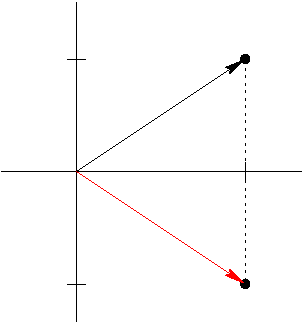
\includegraphics[scale=0.5]{figures/R2-reflectx.pdf}}
\put(1.95,0.4){\tiny{$0$}}
\put(1.95,0.95){\scriptsize{$y$}}
\put(2.8,0.4){\scriptsize{$x$}}
\put(2.7,0.8){\scriptsize{$(a,b)$}}
\put(2.7,0.1){\scriptsize{\alert{$(a,-b)$}}}
\end{picture}
\pause

Let $A$ be the matrix that induces reflection in the $x$-axis.
\pause
If $\lambda$ were an eigenvalue of $A$ and $X$ a corresponding
eigenvector, then $AX=\lambda X$ implies that, geometrically,
\alert{reflecting $X$ in the $x$-axis} is the same as changing
$X$ to a vector parallel to $X$.
\pause
\vspace*{-.2in}
\begin{center}
\alert{How could this be possible?}
\end{center}
\pause
Can you picture what an eigenvector of $A$ would look like?
\end{example}
}
%-------------- end slide -------------------------------%

%-------------- start slide -------------------------------%
\frame{
\begin{example}[continued]
\begin{picture}(4,1.1)
\put(1.4,0){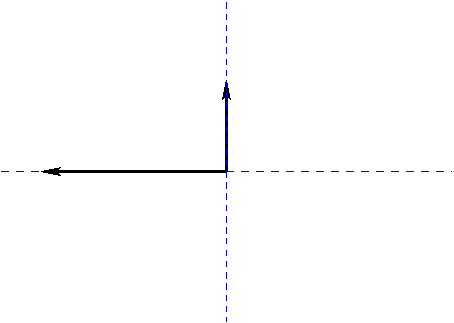
\includegraphics[scale=0.5]{figures/eigenvectors-1.pdf}}
\put(2.0,0.95){\textcolor{blue}{{\scriptsize{$y$}}}}
\put(2.8,0.4){\textcolor{blue}{{\scriptsize{$x$}}}}
\end{picture}
\pause
\begin{itemize}
\item The reflection of 
$\left[\begin{array}{r} -2 \\ 0 \end{array}\right]$
in the $x$-axis is
$\left[\begin{array}{r} -2 \\ 0 \end{array}\right]$,
\pause
\alert{so $\left[\begin{array}{r} -2 \\ 0 \end{array}\right]$
is an eigenvector of $A$ that corresponds to
the eigenvalue $\lambda=1$.}
\pause
\item The reflection of 
$\left[\begin{array}{r} 0 \\ 1 \end{array}\right]$
in the $x$-axis is
$\left[\begin{array}{r} 0 \\ -1 \end{array}\right]$,
\pause
\alert{so $\left[\begin{array}{r} 0 \\ 1 \end{array}\right]$
is an eigenvector of $A$ that corresponds to
the eigenvalue $\lambda=-1$.}
\end{itemize}
\pause
This makes sense, since we know that reflection in the $x$-axis
is induced by the matrix
\[ A=\left[\begin{array}{rr} 1 & 0 \\ 0 & -1 \end{array}\right],\]
\vspace*{-.05in}
which has eigenvalues $1$ and $-1$.
\end{example}
}
%-------------- end slide -------------------------------%

%-------------- start slide -------------------------------%
\frame{
\begin{example}
In $\RR^2$, reflection in the $y$-axis is a linear
transformation that\newline transforms
$\left[\begin{array}{r} a \\ b \end{array}\right]$ to
$\left[\begin{array}{r} -a \\ b \end{array}\right]$.

\pause
\begin{picture}(4,0.9)
\put(1.1,0){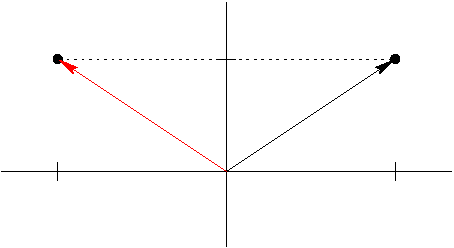
\includegraphics[scale=0.5]{figures/R2-reflecty.pdf}}
\put(1.75,0.15){\scriptsize{$0$}}
\put(1.75,0.8){\scriptsize{$y$}}
\put(2.55,0.15){\scriptsize{$x$}}
\put(2.5,0.6){\scriptsize{$(a,b)$}}
\put(0.88,0.6){\scriptsize{\alert{$(-a,b)$}}}
\end{picture}
\pause

Let $A$ be the matrix that induces reflection in the $y$-axis.
\pause
If $\lambda$ were an eigenvalue of $A$ and $X$ a corresponding
eigenvector, then $AX=\lambda X$ implies that, geometrically,
\alert{reflecting $X$ in the $y$-axis} is the same as changing
$X$ to a vector parallel to $X$.
\end{example}
}
%-------------- end slide -------------------------------%

%-------------- start slide -------------------------------%
\frame{
\begin{example}[continued]
\begin{picture}(4,1.1)
\put(1.4,0){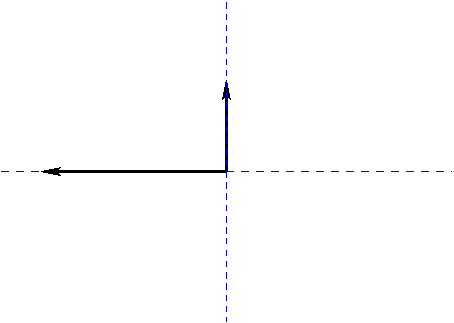
\includegraphics[scale=0.5]{figures/eigenvectors-1.pdf}}
\put(2.0,0.95){\textcolor{blue}{{\scriptsize{$y$}}}}
\put(2.8,0.4){\textcolor{blue}{{\scriptsize{$x$}}}}
\end{picture}
\pause
\begin{itemize}
\item The reflection of
$\left[\begin{array}{r} -2 \\ 0 \end{array}\right]$
in the $y$-axis is
$\left[\begin{array}{r} 2 \\ 0 \end{array}\right]$,
\pause
\alert{so $\left[\begin{array}{r} -2 \\ 0 \end{array}\right]$
is an eigenvector of $A$ that corresponds to
the eigenvalue $\lambda=-1$.}
\pause
\item The reflection of
$\left[\begin{array}{r} 0 \\ 1 \end{array}\right]$
in the $y$-axis is
$\left[\begin{array}{r} 0 \\ 1 \end{array}\right]$,
\pause
\alert{so $\left[\begin{array}{r} 0 \\ 1 \end{array}\right]$
is an eigenvector of $A$ that corresponds to
the eigenvalue $\lambda=1$.}
\end{itemize}
\pause
This makes sense, since we know that reflection in the $y$-axis
is induced by the matrix
\[ A=\left[\begin{array}{rr} -1 & 0 \\ 0 & 1 \end{array}\right],\]
\vspace*{-.05in}
which has eigenvalues $1$ and $-1$.
\end{example}
}
%-------------- end slide -------------------------------%

%-------------- start slide -------------------------------%
\frame{
\begin{example}
Reflection in the line $y=x$ is a linear transformation that \newline
transforms
$\left[\begin{array}{r} a \\ b \end{array}\right]$ to
$\left[\begin{array}{r} b \\ a \end{array}\right]$.

\begin{picture}(4,1.5)
\put(1.4,0){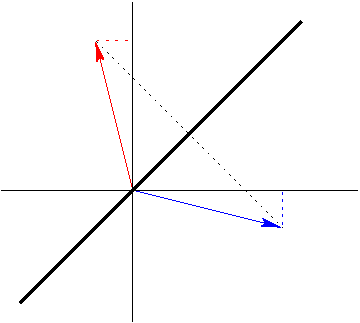
\includegraphics[scale=0.75]{figures/eigenvectors-2.pdf}}
\put(2.85,0.45){\textcolor{blue}{{\scriptsize{$(a,b)$}}}}
\put(1.55,1.4){\textcolor{red}{{\scriptsize{$(a,b)$}}}}
\put(3.2,0.63){\scriptsize{$x$}}
\put(2.1,1.5){\scriptsize{$y$}}
\put(2.8,1.3){\scriptsize{$y=x$}}
\end{picture}
\pause

Let $A$ be the matrix that induces reflection in the line $y=x$.
\pause
If $\lambda$ were an eigenvalue of $A$ and $X$ a corresponding
eigenvector, then $AX=\lambda X$ implies that, geometrically,
\alert{reflecting $X$ in the $y$-axis} is the same as changing
$X$ to a vector parallel to $X$.
\end{example}
}
%-------------- end slide -------------------------------%

%-------------- start slide -------------------------------%
\frame{
\begin{example}[continued]

\begin{picture}(4,1.6)
\put(1.4,0){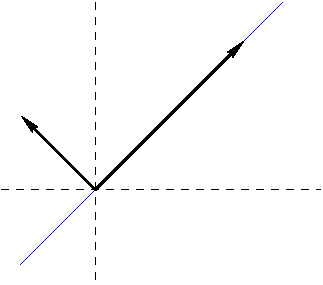
\includegraphics[scale=0.75]{figures/eigenvectors-3.pdf}}
%\put(2.85,0.45){\textcolor{blue}{{\scriptsize{$(a,b)$}}}}
%\put(1.55,1.4){\textcolor{red}{{\scriptsize{$(a,b)$}}}}
%\put(3.2,0.63){\scriptsize{$x$}}
%\put(2.1,1.5){\scriptsize{$y$}}
%\put(2.8,1.3){\scriptsize{$y=x$}}
\end{picture}
\pause

\begin{itemize}
\item The reflection of
$\left[\begin{array}{r} 2 \\ 2 \end{array}\right]$
in the line $y=x$ is
$\left[\begin{array}{r} 2 \\ 2 \end{array}\right]$,
\pause
\alert{so $\left[\begin{array}{r} 2 \\ 2 \end{array}\right]$
is an eigenvector of $A$ that corresponds to
the eigenvalue $\lambda=1$.}
\pause
\item The reflection of
$\left[\begin{array}{r} -1 \\ 1 \end{array}\right]$
in the line $y=x$ is
$\left[\begin{array}{r} 1 \\ -1 \end{array}\right]$,
\pause
\alert{so $\left[\begin{array}{r} -1 \\ 1 \end{array}\right]$
is an eigenvector of $A$ that corresponds to
the eigenvalue $\lambda=-1$.}
\end{itemize}
\pause
Therefore, $1$ and $-1$ are eigenvalues of $A$.
\end{example}
}
%-------------- end slide -------------------------------%

%-------------- start slide -------------------------------%
\frame{
\begin{alertblock}{$\RR^2$: Reflections in lines through the origin}
In $\RR^2$, if $y=mx$ is a line through the origin, then
reflection in the line $y=mx$ is a linear transformation.
\pause
Let $X$ be a vector in $\RR^2$ with tail at the origin.
\smallskip

\pause
\textcolor{blue}{If $A$ is the matrix that induces reflection in
the line $y=mx$}, then 
\pause
\begin{itemize}
\item the reflection of a vector $X$ 
that is \alert{parallel} to $y=mx$ is simply $X$;
\pause
\item the reflection of a vector $X$ 
that is \alert{perpendicular} to $y=mx$ is $-X$.
\pause
\end{itemize}
Therefore, $1$ and $-1$ are eigenvalues of $A$; 
\pause
in fact, these are the only two eigenvalues of $A$ and
each has multiplicity one.  
\pause
This follows from the fact that $A$ is a $2\times 2$ 
matrix, so it's characteristic polynomial has degree two.
\end{alertblock}
}
%-------------- end slide -------------------------------%

%-------------- start slide -------------------------------%
\frame{
\begin{example}[Rotation through $\pi$]
We denote by
\alert{$R_{\pi}:\RR^2\to\RR^2$}
counterclockwise rotation about the origin through an angle
of $\pi$.
\pause
\begin{picture}(4,1.75)
\put(1.3,0.1){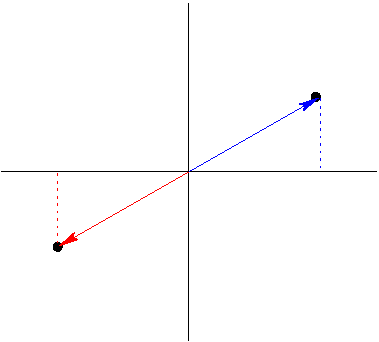
\includegraphics[scale=0.7]{figures/R2-rotate-pi.pdf}}
\put(2.25,0.75){\scriptsize{$0$}}
\put(2.05,1.6){\scriptsize{$y$}}
\put(3.0,0.75){\scriptsize{$x$}}
\put(2.85,1.22){\scriptsize{$(a,b)$}}
\put(1.0,0.5){\scriptsize{\alert{$(-a,-b)$}}}
\end{picture}
\pause

$R_{\pi}$ is a linear transformation that transforms
$X$ to $-X$.
\pause
\medskip

Let $A$ denote the matrix that induces rotation through $\pi$.
\pause
Then $AX=-X$ for every nonzero vector $X$, 
\pause
meaning that 
\alert{every nonzero vector of $\RR^2$ is an eigenvector of
$A$ corresponding to the eigenvalue $\lambda=-1$.}
\end{example}
}
%-------------- end slide -------------------------------%

%-------------- start slide -------------------------------%
\frame{
\begin{example}[Rotation through $\pi/2$]
We denote by
\alert{$R_{\pi/2}:\RR^2\to\RR^2$}
counterclockwise rotation about the origin through an angle
of $\pi/2$.
\pause
\begin{picture}(4,1.75)
\put(1.3,0.1){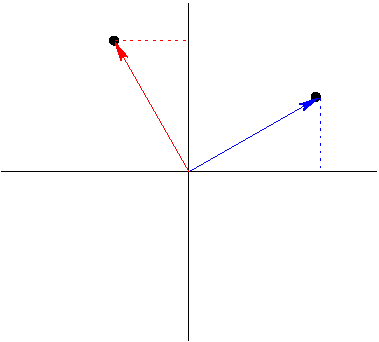
\includegraphics[scale=0.7]{figures/R2-rotate-halfpi.pdf}}
\put(2.25,0.75){\scriptsize{$0$}}
\put(2.05,1.6){\scriptsize{$y$}}
\put(3.0,0.75){\scriptsize{$x$}}
\put(2.85,1.22){\scriptsize{$(a,b)$}}
\put(1.4,1.5){\scriptsize{\alert{$(-b,a)$}}}
\end{picture}
\pause

$R_{\pi}$ is a linear transformation that
transforms
$\left[\begin{array}{r} a \\ b \end{array}\right]$ to
$\left[\begin{array}{r} -b \\ a \end{array}\right]$.
\pause

\alert{Notice that there is no nonzero vector $X$ that can be rotated
through an angle of $\pi/2$ to produce a vector parallel to $X$.}
\pause
Therefore, $A$ has no \alert{real} eigenvalues.
\end{example}
}
%-------------- end slide -------------------------------%

%-------------- start slide -------------------------------%
\frame{
\begin{example}[continued]
Let $A$ denote the matrix that induces rotation through $\pi/2$.
\pause
Then
\[ A= \left[\begin{array}{rr} 0 & -1 \\ 1 & 0 \end{array}\right],\]
\pause
and $c_A(x)=x^2+1$.  
\pause
Therefore, $A$ has complex eigenvalues $i$ and $-i$.
\end{example}
}
%-------------- end slide -------------------------------%

}\end{document}
